\documentclass{beamer}
\usepackage[spanish]{babel}
\usepackage[utf8]{inputenc}
\usepackage{subfig}
\usepackage{pifont}
\usepackage[backend=biber,style=numeric-comp,sorting=none]{biblatex}

\usetheme{Antibes}

% Configuraciones generales
\title{Predictor de Incendios Forestales}
\author{Francisco Muñoz G.}
\institute{
Facultad de Ciencias Físicas y Matemáticas\\
Universidad de Chile
}
\date{22 de junio de 2020}
\logo{
\includegraphics[height=1.7cm]{presentaciones/img/logo solo ingenieria.jpg}}

% Inicio del documento
\begin{document}
% Portada
\frame{\titlepage}

% Tabla de contenidos
\AtBeginSection[]
{
\begin{frame}
    \frametitle{Tabla de Contenidos}
    \tableofcontents[currentsection]
\end{frame}
}
\section{Presentación}
% Interés en el medio ambiente desde muy pequeño
\begin{frame}{Interés en el medio ambiente}
% Imagen de niño pensando
\begin{figure}
    \centering
    \includegraphics[width=0.85\textwidth]{presentaciones/img/01niño_pensando.jpg}
\end{figure}
\end{frame}

% Formas en que pueda ayudar a combatir el cambio climático desde mi área
\begin{frame}{Formas de ayudar}
    \begin{block}{Pregunta: ¿Cómo puedo ayudar a combatir el cambio climático?}
    Quisiera ayudar haciendo lo que más me gusta:
    \begin{itemize}
        \item Matemáticas
        \item Computación
    \end{itemize}
    %   ML y cambio climático
    Y más especificamente: Usar ML para ayudar al medio ambiente.
    \end{block}
\end{frame}

\section{Tema Escogido: Incendios Forestales}
% ¿Por qué escoger incendios Forestales?
\begin{frame}{¿Por qué escoger incendios forestales?}
%    Diversos incendios han ocurrido en el último tiempo
Diversos incendios han ocurrido en el mundo en el último tiempo:
    \begin{figure}
        \subfloat[Amazonas]{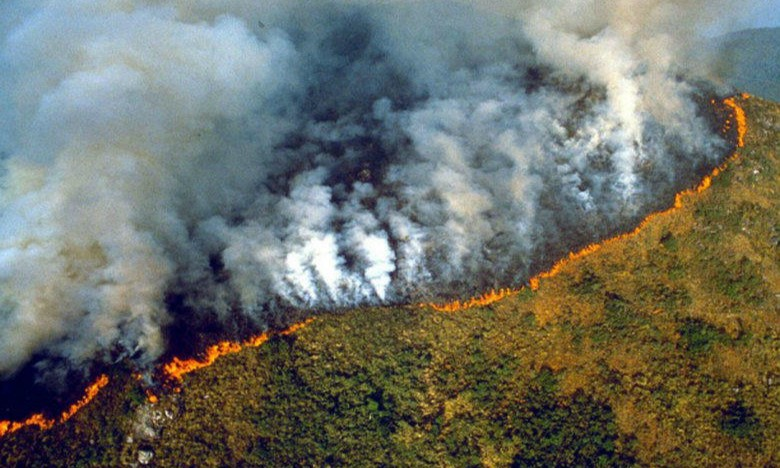
\includegraphics[width=0.3\textwidth]{presentaciones/img/02amazonas.jpg}}\
        \subfloat[Chile]{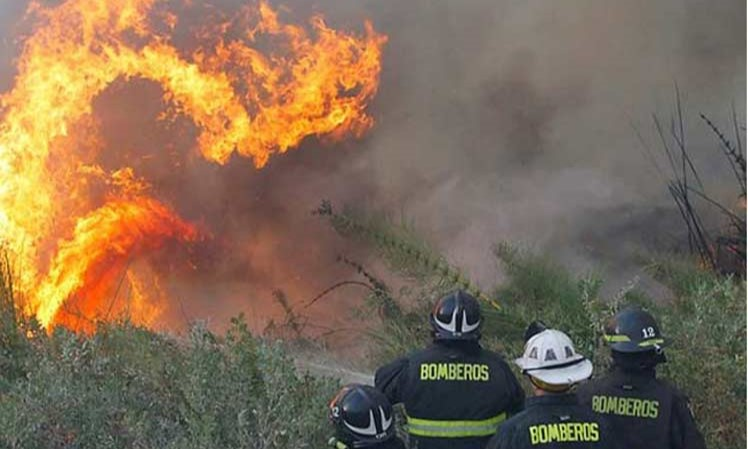
\includegraphics[width=0.3\textwidth]{presentaciones/img/03chile.jpg}}\
        \subfloat[Australia]{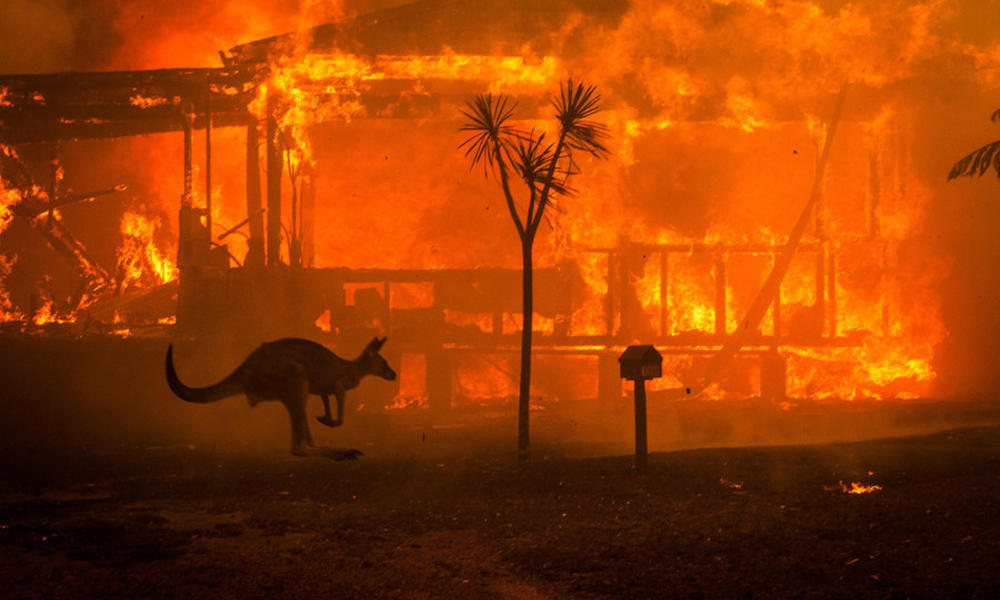
\includegraphics[width=0.3\textwidth]{presentaciones/img/04australia.jpg}}
    \end{figure}
\end{frame}
%    Querer ayudar a los bomberos a combatir los incendios forestales
\begin{frame}{Ayudar a los bomberos!}
    \begin{figure}
        \centering
        \includegraphics[width=0.85\textwidth]{presentaciones/img/05bomberos.jpg}
    \end{figure}
\end{frame}
%    ¿Background? Ninguno.

\section{Posibles Preguntas}
% Dada la geografía y fecha (y quizás otras características que no esté considerando), ¿Cuál será la causa de un incendio?
% Dada la geografía y datos meteorológicos (y quizás otras características que no esté considerando), ¿Es posible predecir la extensión de un incendio a través del tiempo?
\begin{frame}{Posibles preguntas}
    \begin{enumerate}
        \item Dada la geografía y fecha (y quizás otras características que no esté considerando), ¿Cuál será la causa de un incendio? 
        \item Dada la geografía y datos meteorológicos (y quizás otras características que no esté considerando), ¿Es posible predecir la extensión de un incendio a través del tiempo?
    \end{enumerate}
\end{frame}

\begin{frame}{Ventajas y desventajas}
    Ventajas de la \textbf{primera pregunta}:
    \begin{itemize}
        \item[\ding{51}] Se puede responder a través de los \textit{datasets} que tenemos.
    \end{itemize}
    Desventajas:
    \begin{itemize}
        \item[\ding{55}] Es una pregunta más aburrida que la segunda :(
    \end{itemize}
    
    Ventajas de la \textbf{segunda pregunta}:
    \begin{itemize}
        \item[\ding{51}] Es una pregunta bkn y que podría llegar a ser útil.
    \end{itemize}
    Desventajas:
    \begin{itemize}
        \item[\ding{55}] Necesito cruzar los \textit{datasets} con datos meteorológicos.
    \end{itemize}
\end{frame}

\section{Datasets}
% CONAF
\begin{frame}{CONAF}
    % Insertar imagen de CONAF
    \begin{figure}
        \centering
        \subfloat{
\includegraphics[scale=0.09]{presentaciones/img/07conaf.png}}\
        \subfloat{
\includegraphics[width=0.5\textwidth]{presentaciones/img/08conaf2.png}}
    \end{figure}
\end{frame}

% Ventajas y desjentajas
\begin{frame}{Ventajas y Desventajas}
    %    Ventajas:
    %       * Es chileno!
    %       * Tiene los datos necesarios para la primera pregunta
    Ventajas
    \begin{itemize}
        \item[\ding{51}] Es chileno!
        \item[\ding{51}] Tiene los datos necesarios para la primera pregunta
    \end{itemize}
    
    %    Desventajas:
    %       * Tiene pocos datos (comparativamente)
    %       * Está en Excel
    %       * Hay tablas por cada año que no sigue un estándar
    %       * Tablas muy segregadas: Tomará tiempo de más trabajarlas
    Desventajas
    \begin{itemize}
        \item[\ding{55}] Tiene pocos datos (comparativamente).
        \item[\ding{55}] Está en Excel.
        \item[\ding{55}] Hay tablas por cada año, que además no siguen su propio estándar.
        \item[\ding{55}] Tablas muy segregadas: Tomará más tiempo trabajarlas.
    \end{itemize}
\end{frame}

% Kaggle
\begin{frame}{Kaggle: 1.88 Million US Wildfires}
    \begin{figure}
        \centering
        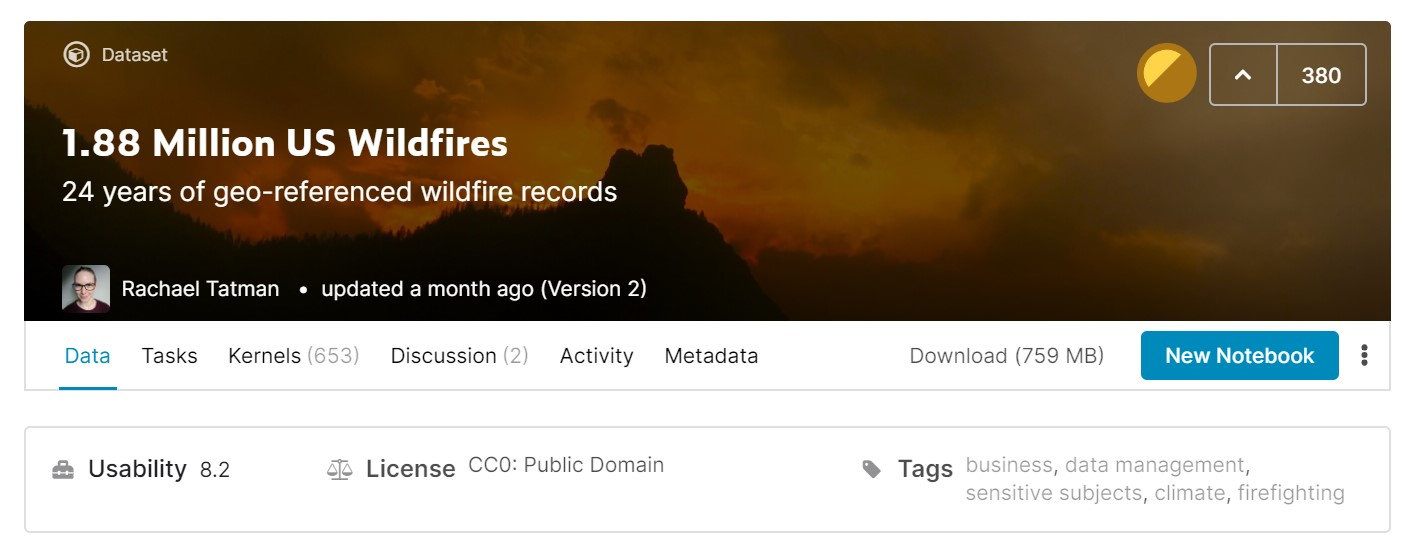
\includegraphics[width=\textwidth]{presentaciones/img/06kaggle.jpg}
    \end{figure}
\end{frame}

% Ventajas y desventajas
\begin{frame}{Ventajas y Desventajas}
%    Ventajas:
%       * Bastantes datos (excesivos diría yo)
%       * Tiene los datos necesarios para la primera pregunta
    Ventajas:
    \begin{itemize}
        \item[\ding{51}] Bastantes datos
        \item[\ding{51}] Tienen los datos necesarios para la primera pregunta
    \end{itemize}
    
%    Desventajas:
%       * Es gringo :c
%       * Muchos datos :c
%       * Dataset muy pesado
    Desventajas:
    \begin{itemize}
        \item[\ding{55}] Es gringo :c
        \item[\ding{55}] Muchos datos :c
        \item[\ding{55}] Dataset muy pesado
    \end{itemize}
\end{frame}



\end{document}